\begin{figure}[t]
\centering
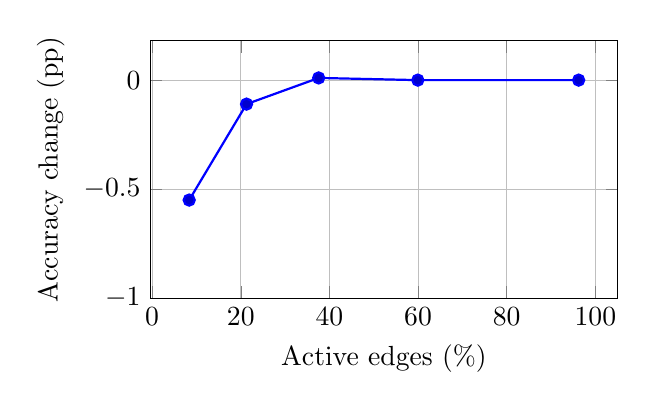
\begin{tikzpicture}
\begin{axis}[width=0.62\textwidth, height=0.4\textwidth, xlabel={Active edges (\%)}, ylabel={Accuracy change (pp)}, grid=both, ymin=-1.0, ymax=0.18]
\addplot+[mark=*, thick] coordinates {(96.23,0.00) (59.94,-0.00) (37.57,0.01) (21.30,-0.11) (8.36,-0.55)};
\end{axis}
\end{tikzpicture}
\caption{Bounded-error event propagation: accuracy change against the fraction of edges that emit, averaged over 56 trained sparse-brain configurations. Propagating one fifth of the edges costs about a tenth of a point.}
\label{fig:theta}
\end{figure}
